%%%%%%%%%%%%%%%%%%%%%%%%%%%%%%%%%%%%%%%%%
% University/School Laboratory Report
% LaTeX Template
% Version 3.0 (4/2/13)
%
% This template has been downloaded from:
% http://www.LaTeXTemplates.com
%
% Original author:
% Linux and Unix Users Group at Virginia Tech Wiki
% (https://vtluug.org/wiki/Example_LaTeX_chem_lab_report)
%
% License:
% CC BY-NC-SA 3.0 (http://creativecommons.org/licenses/by-nc-sa/3.0/)
%
%%%%%%%%%%%%%%%%%%%%%%%%%%%%%%%%%%%%%%%%%

%----------------------------------------------------------------------------------------
%   PACKAGES AND DOCUMENT CONFIGURATIONS
%----------------------------------------------------------------------------------------

\documentclass[12pt, a4paper, ]{article} %fleqn - equ do lewej

\usepackage[utf8]{inputenc}
\usepackage[T1]{fontenc}
\usepackage[MeX]{polski}

\usepackage{siunitx} % Provides the \SI{}{} command for typesetting SI units

\usepackage{graphicx} % Required for the inclusion of images

\usepackage{amsmath}
\usepackage{amsthm} % Twierdzenia, lematy
%\usepackage{ntheorem} % Theorem styles
\usepackage[ruled]{algorithm2e}
\usepackage{hyperref}
\usepackage[section]{placeins}
\usepackage{courier} % font komputerowy \texttt
\usepackage{calc} % do wyliczania długości (wyrównywanie description)
\usepackage{enumitem} % (wyrównywanie description)
\usepackage{pdfpages}


\setlength\parindent{12pt} %  0 -> Removes all indentation from paragraphs
\setlength\parskip{1ex plus 0.5ex minus 0.2ex}

%\renewcommand{\labelenumi}{\alph{enumi}.} % Make numbering in the enumerate
                                    %environment by letter rather than number (e.g. section 6)
\usepackage{lmodern}
%\usepackage{times} % Uncomment to use the Times New Roman font

% Styl stron.
\pagestyle{plain}
\textheight 26cm
\topmargin -0.5cm
\headheight 0cm
\headsep 0cm
\textwidth 16.5cm
\oddsidemargin -0.5cm
%\parindent 0mm

%----------------------------------------------------------------------------------------
%   THEOREMS
%----------------------------------------------------------------------------------------

\newtheorem{definicja}{Definicja}
\newtheorem{obserwacja}{Obserwacja}
%----------------------------------------------------------------------------------------
%   DOCUMENT INFORMATION
%----------------------------------------------------------------------------------------

\title{Izomorfizm grafów \\ GIS \\ Sprawozdanie 1} % Title

\author{Monika \textsc{Woźniak} \and Paweł \textsc{Szynkiewicz}} % Author name

\date{\today} % Date for the report

\begin{document}


\maketitle % Insert the title, author and date

\begin{center}
\begin{tabular}{l r}
Prowadzący projekt: & mgr inż. Łukasz Błaszczyk % Instructor/supervisor
\end{tabular}
\end{center}

%----------------------------------------------------------------------------------------
%   SECTION 1
%----------------------------------------------------------------------------------------

\section{Problem izomorfizmu grafów}

Grafy $G_{X}=(V_{X}, E_{X})$ i~$G_{Y}=(V_{Y}, E_{Y})$ są izomorficzne wtedy i
tylko wtedy, gdy istnieje co najmniej jedno przekształcenie wzajemnie
jednoznaczne; zbiorów wierzchołków $f \colon V_{X} \rightarrow V_{Y}$
oraz zbiorów krawędzi $g \colon E_{X} \rightarrow E_{Y}$
zachowujące relację incydencji krawędzi (albo przylegania wierzchołków), tzn.\
takie że $(v,w) \in E_{X}$ wtedy i tylko wtedy, gdy $(f(v),f(w)) \in E_{Y}$.

Grafy izomorficzne mają identyczną strukturę, różnią się tylko etykietami
wierzchołków. Rozpatrywane będą tylko grafu skierowane. W~ogólności, każdy graf
nieskierowany da się przekształcić w graf skierowany, zamieniając każdą krawędź w
grafie nieskierowanym na dwie krawędzie o przeciwnych zwrotach. Grafy
nieskierowane są izomorficzne, gdy otrzymane z nich grafy skierowane są
izomorficzne.

\paragraph*{Warunki konieczne, jakie muszą spełniać grafy izomorficzne to:}
\begin{itemize}
    \item Jednakowa liczba wierzchołków i~krawędzi.
    \item Ten sam rozkład stopni wierzchołków -- izomorficzne mogą być tylko
        wierzchołki o tych samych stopniach.
    \item Wierzchołki sąsiadujące  z wierzchołkami izomorficznymi muszą mieć
        identyczny rozkład stopni.
    \item Grafy muszą mieć taką samą liczbę cykli o identycznej długości~\cite[str.~49]{b:GiS:2013}.
       % bibl [1]
\end{itemize}

W ogólnym przypadku, bez dodatkowych założeń, stwierdzenie izomorfizmu grafów należy do
klasy problemów NP trudnych. W praktyce, dla większości grafów możliwe
jest ograniczenia przeszukiwanego zbioru wszystkich przyporządkowań.
Ograniczenia te wynikają bezpośrednio z~warunków koniecznych jakie muszą
spełniać grafy izomorficzne.

\section{Metoda powrotów}

Problem rozstrzygania izomorfizmu grafów skierowanych rozwiązywany będzie za
pomocą algorytmu powrotów~(ang.\ \textit{backtracking}). Jest to ogólna strategia
konstruowania optymalnych rozwiązań ponadwielomianowych, gdy nie znane jest
rozwiązanie wielomianowe, lub gdy takie rozwiązanie nie istnieje.

\subsection{Opis algorytmu}

Rozpatrywana jest przestrzeń stanów, gdzie stan to pewne przyporządkowanie węzłów z~podzbioru
wierzchołków grafu $G_{X}$, węzłom z~podzbioru wierzchołków grafu $G_{Y}$. Stan jest sytuacją
stanowiącą rozwiązanie problemu albo mogącą prowadzić do rozwiązania poprzez przechodzenie
z~jednego stanu w~drugi.

Aby znaleźć rozwiązanie, konieczne jest przeszukanie przestrzeni stanów,
przechodząc z jednego stanu w drugi, aż do uzyskania stanu określającego
rozwiązanie problemu. Ponieważ dla każdego stanu może istnieć wiele
dopuszczalnych ruchów, czyli wiele stanów, do których można dojść, możliwy jest
wybór złego posunięcia. Jeżeli wykonano zły ruch i obecny stan nie może
prowadzić do rozwiązania (nie osiągnięto poprawnego rozwiązania i nie ma więcej
dopuszczalnych posunięć), konieczne jest cofnięcie się do ostatniego stanu,
w~którym istnieje możliwość wykonania poprawnego przejścia. Metoda powrotów
wymaga zapamiętania wszystkich wykonanych ruchów, czy też wszystkich
odwiedzonych stanów.

Przestrzeń wszystkich, możliwych wzajemnych przyporządkowań wierzchołków dwóch
n-wierz\-choł\-ko\-wych grafów skierowanych składa się z~$ n! $ elementów. Ze względu
na zależność $ n! $ naiwny algorytm powrotów ma dużą złożoność i jest
niezadowalający. Do rozwiązania problemu zastosowana będzie metoda powrotów z
ograniczeniami. Gałęzie drzewa wyszukiwania, nie prowadzące do poprawnego
przyporządkowania, będą zawczasu odcinane.

\vspace{10 pt}
\begin{definicja}\label{def:WejWyj}
    \mbox{}
    \begin{itemize}
        \item[(i)] \textbf{Wejściowość} wierzchołka grafu skierowanego
            odpowiada liczbie krawędzi \textbf{wchodzących} do tego wierzchołka.
        \item[(ii)] \textbf{Wyjściowość} wierzchołka grafu skierowanego
            odpowiada liczbie krawędzi \textbf{wychodzących} z tego wierzchołka.
    \end{itemize}
\end{definicja}


\vspace{1 pt}
\begin{obserwacja}\label{obs:WejWyj}
    Wierzchołek z grafu $G_{X}$ może być przyporządkowany wierzchołkowi z grafu
    $G_{Y}$ tylko, gdy ich wejściowość i wyjściowość są sobie równe.
\end{obserwacja}
% TODO Na podstawie tej obserwacji dokonywane jest ograniczenie możliwych przyporządkowań.
\vspace{3 pt}

\subsection{Założenia algorytmu}
Dane są dwa spójne grafy skierowane:
\[
    \begin{array}{l}
        G_{X} = (V_{X}, E_{X})\\
        G_{Y} = (V_{Y}, E_{Y})
    \end{array}
\]
należy rozstrzygnąć, czy grafy są izomorficzne, $G_{X} \cong G_{Y}$. Zakładamy,
że oba grafy mają taką samą liczbę wierzchołków i taką samą liczbę krawędzi
($|V_{X}| = |V_{Y}|$ i $|E_{X}| = |E_{Y}|$). Dodatkowo multizbiory zawierający
wejściowości, odpowiednio wyjściowości wierzchołków grafu $G_{X}$, odpowiada
multizbiorom wejściowości i wyjściowości wierzchołków grafu $G_{Y}$
(obs.~\ref{obs:WejWyj}) W~przypadku nie spełnienia założeń, grafy $G_{X}$ i
$G_{Y}$ nie są izomorficzne. Jeden z grafów, (załóżmy, że $G_{X}$) przyjmuje
się za graf odniesienia. Niech $G_{X}(k)$ oznacza podgraf grafu $G_{X}$
indukowany przez zbiór wierzchołków $\{1, 2 \ldots k\},\hspace{0.5 em}0 \leq k
\leq n$~\cite[str.~362]{b:AlgKomb:1985}.


\subsection{Kroki algorytmu}

Do rozstrzygnięcia, czy $G_{X} \cong G_{Y}$ użyta zostanie metoda powrotów,
gdzie stanem jest przyporządkowanie wierzchołków grafu $G_{X}(k)$ i pewnego
podgrafu grafu $G_{Y}$. $G_{X}(0)$ jest izomorficzny z pustym pografem $G_{Y}$.
Po $k$ krokach znaleziono podgraf $G_{Y}$ złożony z wierzchołków $S \subseteq
V_{Y}$ izomorficzny z $G_{X}(k)$. Następnie próbuje się rozszerzyć izomorfizm
na graf $G_{X}(k+1)$, wybierając wierzchołek $v \in V_{Y} - S$, który może być
przyporządkowany wierzchołkowi $k+1 \in V_{X}$. Jeżeli uda się znaleźć taki
wierzchołek, przyporządkowane zostaje zapamiętane,  izomorfizm próbuje się
rozszerzyć na $G_{X}(k+2)$. W przypadku, gdy nie istnieje taki wierzchołek $v$,
powraca się do przyporządkowania z $G_{X}(k-1)$ i próbuje się wybrać inny
wierzchołek który można przyporządkować węzłowi $k \in V_{X}$. Proces
kontynuuje się aż do momentu, gdy $G_{X}(n) = G_{X}$, co jest jednoznaczne
stwierdzeniu, że grafy $G_{X}$ i $G_{Y}$ są izomorficzne lub, gdy proces
powróci do $G_{X}(0)$ co oznacza, że grafy nie są izomorficzne, $G_{X}
\not\cong G_{Y}$.

\begin{algorithm}[tp]
    \RestyleAlgo{ruled}
    \SetAlgoLined\DontPrintSemicolon{}
    \caption{Sprawdzanie izomorfizmu grafów skierowanych}
    \SetKwFunction{fIsomorph}{\textsc{Isomorph}}
    \SetKwFunction{fMatch}{\textsc{Match}}
    \SetKwProg{pIsomorph}{Procedure}{}{}
    \SetKwProg{pMatch}{Procedure}{}{}
    \KwData{$G_{X}$, $G_{Y}$, flag k\;}
    \KwResult{czy $G_{X} \cong G_{Y}$, przy przyporządkowaniu $i \leftrightarrow f_{i}$}
    \;
    flag $\leftarrow$ \textit{false}\;
    k $\leftarrow$ 0\;
    \fIsomorph{$\emptyset$}\;
    \eIf{flag}{
        $G_{X} \cong G_{Y}$\;
        przyporządkowanie: $i \leftrightarrow f_{i}$\;
    }{
        $G_{X} \not\cong G_{Y}$\;
    }
    \;
    \pIsomorph{\fIsomorph{S}}{
        k $\leftarrow \text{k} + 1$\;
        \If{$S = V_{Y}$}{
            flag $\leftarrow$ \textit{true}\;
        }
        \For{$v \in V_{Y} - S$ \textbf{and not} flag}{
            \If{\fMatch{$v$}}{
                $f_{k} \leftarrow v$\;
                \fIsomorph{S $ \cup \{v\}$}\;
            }
        }
        k $\leftarrow \text{k} - 1$\;
    }
    \;
    \pMatch{\fMatch{}}{
        \eIf{wierzch. $v \in V_{Y} - S$ można przyporządkować wierzch. $k \in V_{X}$}{
            \Return{true}
        }{
            \Return{false}
        }
    }
\end{algorithm}
\clearpage

\subsection{Modyfikacja metody powrotów}

Modyfikacje metody powrotów mają na celu ograniczanie drzewa wyszukiwania.
Gałęzie drzewa, które nie prowadzą do poprawnego przyporządkowania świadczącego
o~izomorfizmie rozpatrywanych grafów, nie powinny być odwiedzane.

\subsubsection{Numerowanie wierzchołków}

W~powyższym algorytmie, wierzchołki grafu $G_X$ mają etykiety z~zakresu ${1
\ldots n}$. Dobre ponumerowanie wierzchołków pozwala na lepsze ograniczenie
przestrzeni przeszukiwania. Metoda numerowania wierzchołków oparta jest na
poniższych heurystykach:

\paragraph{Pierwszy -- najbardziej ograniczony}\mbox{}

Na początku działania algorytmu rozpatrywane powinny być wierzchołki
o~najmniejszej możliwej liczbie przyporządkowań. W~ten sposób drzewo
przeszukiwania nie rozrasta się na wstępie. Częste cofanie się do stanu
$G_X(1)$ byłoby niekorzystne.

\paragraph{Pierwszy -- sąsiadujący}\mbox{}

Aktualnie przyporządkowywany wierzchołek powinien sąsiadować z~jak największą
liczbą wierzchołków przyporządkowanych w~poprzednim kroku. Ogranicza to liczbę
możliwych przyporządkowań, ponieważ nakładane są dodatkowe wymagania na
rozpatrywany wierzchołek.


\paragraph{DFS od najbardziej ograniczonego}\mbox{}

Wykorzystywane jest połączenie obu heurystyk. Warunkiem przyporządkowania
pierwszego wierzchołka jego stopień. Dlatego numerowanie zaczynamy od
wierzchołka $x \in V_X$, takiego że najmniej wierzchołków $v \in V_X$ spełnia
warunek $d^+(x)=d^+(v)$ i~$d^-(x)=d^-(v)$. Kolejne wierzchołki numerowane są
zgodnie z~metodą przeszukiwania zstępującego, czyli \textit{DFS}.

\subsubsection{Stopień wierzchołka}

Wierzchołki można przyporządkować wtedy i~tylko wtedy, gdy ich wejściowości i~wyjściowości
są takie same. Dlatego przy rozpatrywaniu kolejnego wierzchołka grafu $G_X$, pod uwagę
brane będą jedynie takie wierzchołki grafu $G_Y$, które spełniają powyższy warunek i~nie
mają jeszcze przyporządkowania. Zasada ta powinna znacznie ograniczyć drzewo przeszukiwania
w~przypadku większości grafów.


\subsubsection{Warunki początkowe}

Przed zastosowaniem metody powrotów, sprawdzane będą warunki początkowe,
czyli niektóre warunki konieczne jakie muszą spełniać grafy izomorficzne.
\begin{enumerate}
  \item Jednakowa liczba wierzchołków
  \item Jednakowa liczba krawędzi
  \item Taki sam rozkład stopni wierzchołków (wejściowość i~wyjściowość)
\end{enumerate}

\subsection{Poprawność algorytmu}

Algorytm opiera się na metodzie powrotów. Metoda ta polega na przechodzeniu
drzewa przeszukiwania. Każdy węzeł drzewa, reprezentuje dokładnie jedno
unikalne przyporządkowanie wierzchołków grafu $G_X$ wierzchołkom grafu $G_Y$.
Istnieje dokładnie $n!$ takich przyporządkowań, gdzie $n$ to liczba wierzchołków
w~grafach. Metoda powrotów zakończy się po znalezieniu przyporządkowania
będącego izomorfizmem. Zakończy się również, po przejściu całego drzewa
przeszukiwania. Ponieważ drzewo ma określony rozmiar, metoda zawsze się zakończy.


W~przypadku, gdy grafy są izomorficzne, metoda zakończy swoje działanie na
pewnym wierzchołku drzewa przeszukiwania. Wierzchołek ten reprezentuje przyporządkowanie
będącym izomorfizmem grafów. Ponieważ przeglądane są wszystkie węzły drzewa, do
momentu znalezienia izomorfizmu, metoda na pewno znajdzie przyporządkowanie izomorficzne.
Kolejność rozpatrywanych wierzchołków nie ma znaczenia dla poprawnego działania algorytmu.
Wszystkie możliwe drzewa przeszukiwania są równoważne (są ze sobą izomorficzne).


Usprawnienia metody powrotów nie wpływają na poprawność działania algorytmu. W~szczególności
jeżeli dane przyporządkowanie nie spełnia izomorfizmu, to rozszerzenie tego przyporządkowania,
także nie spełnia izomorfizmu. Uznanie, że dany wierzchołek $x \in G_X$ nie może być przyporządkowany
wierzchołkowi $v \in G_Y$ (bo nie spełnia izomorfizmu) oznacza, że odrzucamy
wszystkie przyporządkowania w~których $x$ jest przyporządkowane $v$. Jest to jednoznaczne
odcięciu gałęzi drzewa przeszukiwania, w~której na pewno nie ma rozwiązania problemu
izomorfizmu.
\subsection{Złożoność algorytmu}

Złożoność metody powrotów to $O(n!)$ gdzie $n$ to liczba wierzchołków w~grafie.
W~przypadku pesymistycznym, pierwszy wierzchołek będzie przyporządkowany $n$ razy,
drugi $n - 1$, itd\dots co razem stanowi $n!$ sprawdzonych przyporządkowań.
Należy zaznaczyć, że wprowadzone usprawnienia metody powrotów, oparte są na heurystykach.
Stosuje się je, mając na celu jak największą redukcję drzewa przeszukiwania. Nie oznacza
to jednak, że metody te sprawdzą się w~przypadku wszystkich grafów. Próby obcinania gałęzi
drzewa mogą zakończyć się niepowodzeniem. W~takim przypadku konieczne będzie sprawdzenie wszystkich
lub prawie wszystkich $n!$ możliwych przyporządkowań.

W~praktyce usprawniona metoda powrotów, powinna działać sprawnie dla rozsądnych wymiarów zadania, zwłaszcza dla grafów rzadkich i
grafów o~różnorodnym rozkładzie stopni wierzchołków.

\section{Założenia implementacyjne}

Program zostanie napisany w~języku C++. Możliwe będą dwa scenariusze użycia programu:
\begin{itemize}
  \item Podanie ścieżek do dwóch plików tekstowych z~grafami
  \item Podanie ilości wierzchołków i~gęstości do generowania grafu losowego
\end{itemize}
W~pierwszym przypadku, program rozwiązuje problem izomorfizmu zadany przez użytkownika.
W~drugim, program sam generuje losowe grafy izomorficzne i~rozwiązuje problem ich izomorfizmu.

Grafy w~plikach zapisane są w~reprezentacji list sąsiedztwa. Każda lista zajmuje dokładnie jedną linię.
Aby otrzymać parę losowych grafów izomorficznych w~pierwszym kroku generowany jest graf losowy.
W~drugim, graf jest kopiowany otrzymana kopia poddawana jest losowemu przekształceniu izomorficznemu.

Na wyjściu program zwraca komunikat informujący, czy zadane grafy są izomorficzne, oraz
odpowiadające temu izomorfizmowi przyporządkowanie wierzchołków.



\section{Testy}
W~celu zweryfikowania poprawności i~wydajności powstałego programu, przeprowadzone zostaną
dwie grupy testów.
\subsection{Testy poprawnościowe}
Testy będą służyły weryfikacji wyników zwracanych przez program. Na wejście programu zadawane
będą pliki zawierające reprezentację grafów w~postaci list sąsiedztwa. Pliki zostaną przygotowane
ręcznie. Celem testów będzie sprawdzenie:
\begin{itemize}
  \item Czy program wykryje parę grafów nieizomorficznych
  \item Czy program wykryje parę grafów izomorficznych
  \item W~wypadku grafów izomorficznych, czy program zwróci poprawne
    przyporządkowanie wierzchołków
\end{itemize}
Przygotowane testy sprawdzą, także poprawność działania następujących etapów programu:
\begin{itemize}
  \item Weryfikacji warunków początkowych (koniecznych) izomorfizmu
  \item Metody powrotów
\end{itemize}


\subsection{Testy wydajnościowe}
Testy posłużą ocenie jakości działania programu. Złożoność problemu izomorfizmu
grafów szybko rośnie wraz z~wymiarem zadania. Przeprowadzone testy pomogą przy ocenie
programu, jak i~samej metody powrotów przy rozpatrywaniu izomorfizmu dla grafów
większych rozmiarów.

Grafy do testów, o~danej ilości wierzchołków i~gęstości, będą generowane losowo.
Liczony będzie czas działania programu, w~zależności od ilości wierzchołków i~krawędzi.
Wyniki będą uśredniane.

\section{Program Izomorf}
Program \textbf{Izomorf} służy do weryfikacji izomorfizmu dwóch grafów spójnych, skierowanych.
Program jest napisany w~języku \textit{C++} w~standardzie \textit{C++11}. Został skompilowany
w~środowisku \textit{Linux}, kernel 3.13.6-1.

\subsection{Kod}
Logikę programu stanowią trzy klasy: \texttt{Vertex}, \texttt{Graph}, \texttt{IsomorphismAlgo}.
Funkcja \texttt{main} znajduje się w~pliku \textit{izomorf.cpp}, wykorzystuje funkcje pomocnicze
z~tego pliku do parsowania parametrów wykonania programu.

\subsubsection{Klasa Vertex}
Klasa reprezentuje wierzchołek grafu i~jego listę sąsiedztwa. Obiekt klasy pozwala na:
\begin{itemize}
  \item Dodawanie wierzchołka sąsiedniego.
  \item Iterowanie po liście sąsiedztwa.
  \item Uzyskanie \textit{wejściowości}/\textit{wyjściowości} wierzchołka.
\end{itemize}


\subsubsection{Klasa Graph}
Klasa implementuje graf skierowany w~reprezentacji list sąsiedztwa. Do przechowywania informacji o~listach
wykorzystywane są obiekty klasy \texttt{Vertex}. Klasa \texttt{Graph} to interfejs, który umożliwia
tworzenie przechowywanie grafów. Obiekty klasy \texttt{Graph} umożliwiają.
\begin{itemize}
  \item Dodawania wierzchołków i~krawędzi do grafu.
  \item Iterowanie po wierzchołkach i~krawędziach grafu.
  \item Wczytywanie i~zapisywanie grafu do strumieni danych.
  \item Uzyskanie \textit{wejściowości}/\textit{wyjściowości} wierzchołka grafu.
\end{itemize}

Klasa \texttt{Graph} udostępnia metodę do generowania losowych, spójnych grafów skierowanych.
Istnieje także możliwość tworzenia losowych grafów, które będą izomorficzne do zadanego grafu.


\subsubsection{Klasa IsomorphismAlgo}
Algorytm weryfikacji zaimplementowano za pomocą klasy \texttt{IsomorphismAlgo}. Pozwala to na
przechowywanie w~polach klasy struktur danych wykorzystywanych przez algorytm powrotów. Dzięki
temu kod jest czytelniejszy, ponieważ funkcje nie pobierają dużej ilości parametrów. Jednocześnie
unika się z~korzystania ze zmiennych globalnych.

\vspace{2 em}

Klasa \texttt{IsomorphismAlgo} udostępnia dwie metody publiczne:
\begin{description}[leftmargin=!,labelwidth=\widthof{\bfseries meetsRequirements}]
  \item [\texttt{meetsRequirements}] funkcja sprawdza czy dwa grafy spełniają warunki
    wstępne izomorfizmu grafów.
  \item [\texttt{isIsomorphism}] funkcja sprawdza czy dwa grafy są izomorficzne.
\end{description}

\vspace{2 em}

Można wyróżnić dwa etapy działania klasy \texttt{IsomorphismAlgo}
\begin{enumerate}
    \item inicjalizacja struktur danych.
    \item wywołanie metody powrotów.
\end{enumerate}

Metoda powrotów wykonywana jest w~metodzie \texttt{match}. Funkcja wywoływana jest rekurencyjnie.


\subsection{Instrukcja obsługi}
Program \textbf{Izomorf} należy wywołać z~linii komend z~odpowiednimi parametrami wykonania.
\begin{description}[leftmargin=!,labelwidth=\widthof{\bfseries f FN1 FN2}]
  \item [\texttt{<brak>}] wywołanie programu bez parametrów powoduje
    wyświetlenie pomocy użytkownika.
  \item [\texttt{f FN1 FN2}] po opcji \texttt{f} należy podać ścieżki do dwóch
    plików (\texttt{FN1}, \texttt{FN2}) z~grafami w~rozpoznawanym formacie.
    Program wczytuje oba grafy i~weryfikuje ich izomorfizm.
  \item [\texttt{r V D}] program generuje dwa losowe grafy izomorficzne, o~liczbie
    wierzchołków \texttt{V} i~gęstości krawędzi \texttt{D}. Następnie izomorfizm
  wylosowanych grafów jest weryfikowany. ($0 \leq V \leq 1000$, $D \in (0, 1]$).
  \item [\texttt{t}] opcja \texttt{t} powoduje uruchomienie testów programu i
    wypisanie ich wyniku na konsolę.
\end{description}

Wiadomość pomocnicza, zwracana jest na konsolę, gdy program zostanie wywołany bez
argumentów, lub gdy podane parametry są błędne. Podanie złych parametrów generuje
dodatkowo stosowny komunikat o~błędzie.

\vspace{1 em}

\noindent
\textbf{Format wiadomości pomocniczej:}
\begin{verbatim}
Program do weryfikowania izomorfizmu grafów
IZOMORF [OPCJA] [VAL1] [VAL2]
 OPCJE:
--------------------------------------------------------------------------------
    f <plik z grafem 1> <plik z grafem 2>
          wczytaj grafy z plików i przetestuj ich izomorfizm
--------------------------------------------------------------------------------
    r <V = liczba wierzchołków> <D = gęstość>
          wygeneruj graf dwa izomorficzne grafy losowe o danej ilości
          wierzchołków i gęstości i przetestuj ich izomorfizm
          0 <= V <= 1000, D in (0, 1]
--------------------------------------------------------------------------------
    t
          przeprowadź serię testów
\end{verbatim}

\clearpage
\section{Wyniki testów}
Testy zostały przeprowadzone na maszynie z~systemem operacyjnym \textit{Linux} 64 bit o
z~procesorem \textit{Intel Core Duo} 2GHz i~pamięcią \textit{RAM} 2GiB. Rozmiar
stosu jaki przydzielany funkcji rozszerzono do 20 MB.
\subsection{Wyniki testów poprawnościowych}
Testy poprawnościowe przeprowadzono na ręcznie przygotowanych parach grafów, zapisanych w
plikach w~folderze \emph{tests}. Testy poprawnościowe podzielono na trzy klasy, dla
każdej klasy wykonano po kilka testów:
\begin{enumerate}
  \item Para grafów nie spełnia warunków wstępnych izomorfizmu.
  \begin{itemize}
      \item Para grafów ma różną ilość wierzchołków.
      \item Para grafów ma różną ilość krawędzi.
      \item Para grafów ma różną liczność wierzchołków o~takich samych stopniach.
  \end{itemize}
  \item Para grafów spełnia warunki początkowe, ale nie jest izomorficzna.
  \item Para grafów jest izomorficzna.
\end{enumerate}

\noindent
Każda klasa testów sprawdzała inne zachowanie programu.
\begin{enumerate}[label=Ad. \arabic*]
  \item Program wykrywał grafy nieizomorficzne, już na etapie sprawdzania
    warunków wstępnych.
  \item Grafy przechodziły testy wstępne, ale algorytm wykrywał, że nie są izomorficzne.
  \item Program weryfikował grafy jako izomorficzne.
\end{enumerate}

Program przeszedł pomyślnie wszystkie testy poprawnościowe.
\subsection{Wyniki testów wydajnościowych}
Testy wydajnościowe polegały na weryfikowaniu izomorfizmu dwóch grafów losowych,
które z~założenia były izomorficzne. Sprawdzano szybkość działania programu dla
grafów o~różnej ilości wierzchołków i~krawędzi. Czas wykonania rośnie wykładniczo wraz
ze wzrostem liczby wierzchołków. Dla grafów o~większej ilości krawędzi program działa i
takiej samej ilości wierzchołków, program działa dłużej. Poniższy wykres przedstawia
uśrednione wyniki, przy odrzucaniu skrajnych przypadków.

\begin{figure}[!ht]
    \centering
    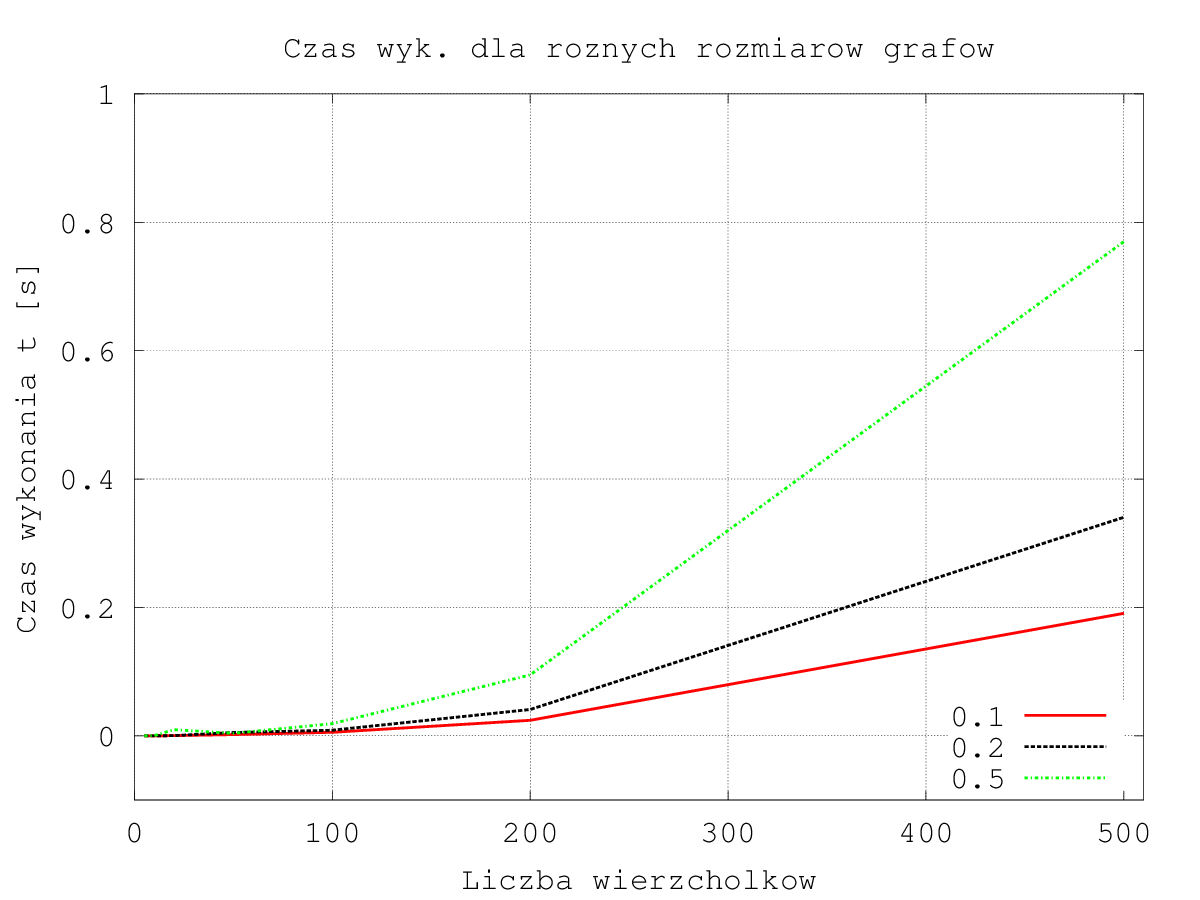
\includegraphics[width=0.8\textwidth]{rys1}
    \caption{Czas wykonania dla różnych rozmiarów grafów, gęstości krawędzi 0.1, 0.2 i~0.5}
    \label{fig:rys1}
\end{figure}

\begin{figure}[!ht]
    \centering
    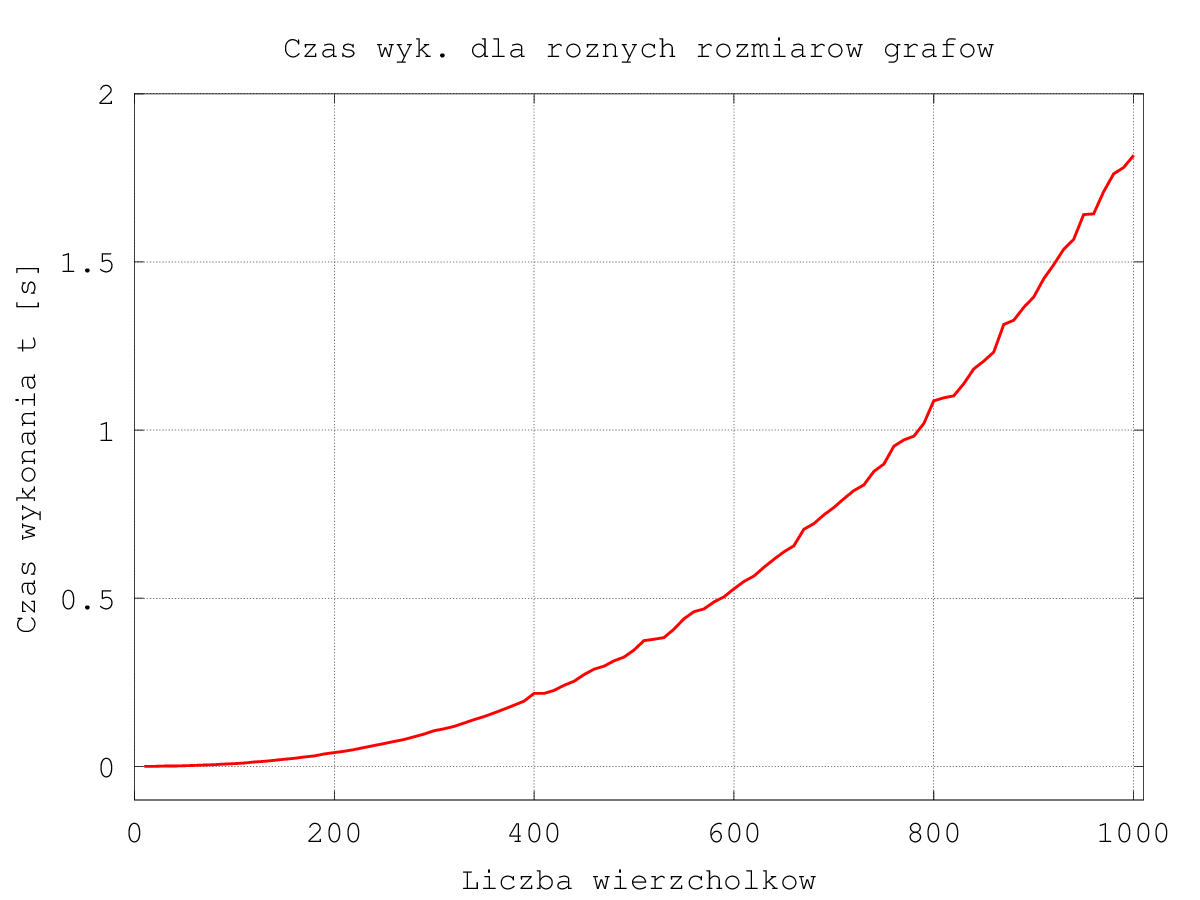
\includegraphics[width=0.8\textwidth]{rys2}
    \caption{Czas wykonania dla różnych rozmiarów grafów}
    \label{fig:rys2}
\end{figure}
\clearpage

\section{Wnioski}
Wykorzystanie metody powrotów, z~dodatkowym obcinaniem gałęzi drzewa przeszukiwań, dawało
zadowalające wyniki. Weryfikowano izomorfizm grafów o~rozmiarach do~2000 wierzchołków. Średni
czas działania metody dla losowych grafów mających 2000 wierzchołków to 5.5 s.
Chociaż problem izomorfizmu grafów jest problemem \emph{NP\dywiz trudnym} metoda powrotów,
wzbogacona o~pewne heurystyki działa sprawnie dla większości wylosowanych grafów.
Trzeba jednak pamiętać, że pesymistyczna złożoność tej metody to dalej $n!$. Podczas testów
na grafach losowych zaobserwowano przypadki, w~których program działał wyraźnie dłużej.
W~skrajnych przypadkach trzeba było przerwać działanie programu. Należy więc
podkreślić, że metoda nie sprawdza się dla wszystkich grafów. Ponieważ
przestrzeń poszukiwań dla złożoności $n!$ rośnie szybko wraz z~wymiarem
zadania, przypadki pesymistyczne mogą okazać się nierozwiązywalne już dla
grafów o~liczbie wierzchołków przekraczającej 20.

Słabą stroną metody może okazać się nie tylko jej złożoność czasowa. Podczas implementacji problemu
zauważono, także problemy związane ze złożonością pamięciową metody. Ponieważ funkcja
weryfikująca izomorfizm wywołuje się rekurencyjnie, dla większych wymiarów zadania dochodziło do
przepełnienia stosu.  Rozwiązaniem tymczasowym było zwiększenie wielkości stosu
w~parametrach systemu (polecenie \texttt{ulimits -s} w~systemie \textit{Linux}).
Być może lepszym rozwiązaniem, byłoby usunięcie rekurencji i~symulowanie stosu
na stercie.


%----------------------------------------------------------------------------------------
%   BIBLIOGRAPHY
%----------------------------------------------------------------------------------------
\bibliographystyle{plain}

\nocite{*}
\bibliography{GIS_spr3}{}
\clearpage

\includepdf[pages=-]{refman.pdf}
\end{document}
